\documentclass[Softwaredesign/Softwaredesign_main.tex]{subfiles}

\begin{document}
\subsection{CoinDetector} \label{sec:CoinDisp}
Våres design krever en måte å oppdage mynter, samt en måte å håndtere mynter etter at de hadde kommet inn i systemet. I denne delen er designet av CoinDetector samt noen valg som ble tatt underveis. 
\\ 
CoinDetector-programvaren består av 2 forskjellige moduler, de er CoinDetector og MotorControl. CoinDetector modulet er hovedlogikken til programvaren, den inneholder state maskinen enabled og disabled som bestemmer om den skal motta eller avise myntene som kommer inn i systemet.
\subsubsection{CoinDetector design valg} 
Ved utformingen av CoinSensor så vi på noen forskjellige tilnærminger. Ideene vi overveide var en slags lyssensor eller en form for bytter som mynten ville trykke ned når den kom inn i systemet, før vi endte opp med det endelige designet med en kortslutning. 
\subsubsection{CoinDetector med kortslutningsdesign} 
\begin{figure}[H]
    \centering
    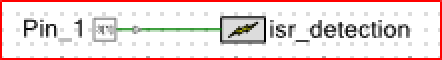
\includegraphics[width=0.5\textwidth]{Softwaredesign/CoinSensor/graphics/TopDesign-CoinDetector.png}
    \caption{PSoC top design CoinDetector}
    \label{fig:CoinDetector_PSoC_Design}
    \end{figure}
Programvaren til detektoren er ganske enkel. Den består av en enkel interrupt. Interruptet deaktiverer fremtidige interrupt, og kaller de riktige funksjonene avhengig av hvilken tilstand dispenseren er i. Hvis dispenseren er i dissabed, kalles den nødvendige motoren for å avvise mynten, reaktiverer interrupts og deretter gå tilbake til å vente. Hvis dispenseren er activated, kaller den de nødvendige motorfunksjonene å akseptere myntene og deretter gå tilbake til å vente. Under ligger et diagram som viser dette.
\begin{figure}[H]
    \centering
    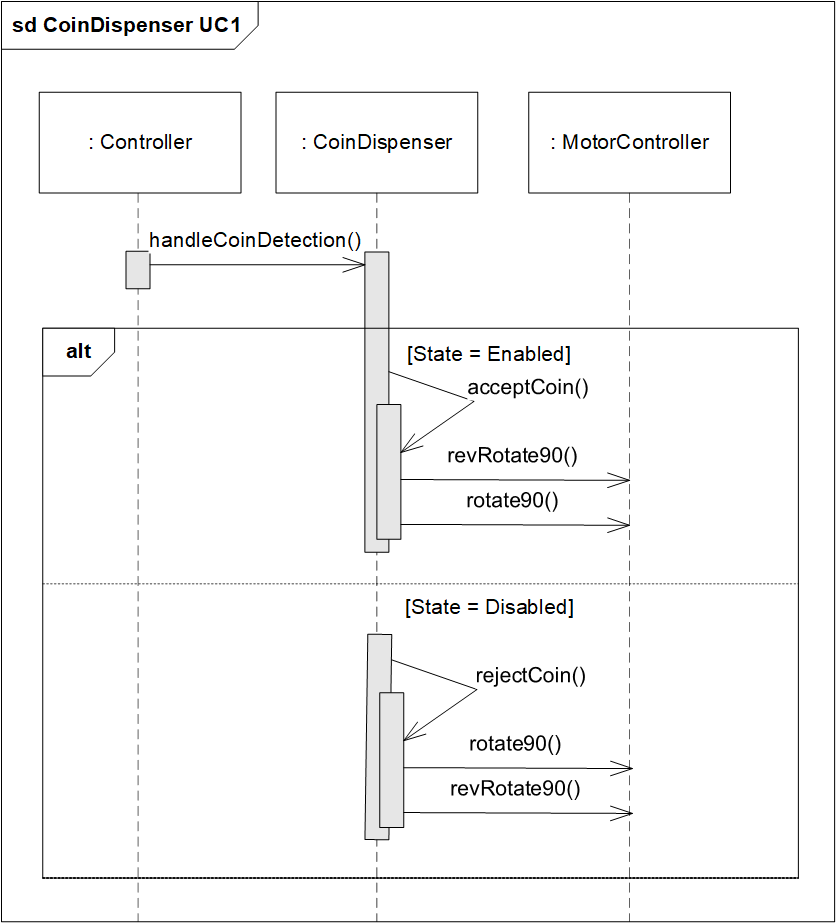
\includegraphics[width=\textwidth]{Softwaredesign/CoinSensor/graphics/sd_CoinDispenser.png}
    \caption{Sekvens diagram som viser coin dispensers funksjonalitet}
    \label{fig:SDCoinDispAPP}
\end{figure}

\end{document}